\section{Suddivisione del lavoro e Prospetto Orario} 

\sectionmark{Suddivisione del lavoro \dots}

Ogni componente del gruppo dovrà ricoprire ogni ruolo almeno una volta nel corso del progetto.
Durante la stessa fase un componente può ricoprire più ruoli, a condizione che le mansioni previste non vadano in conflitto tra loro, ad esempio non si può verificare il proprio lavoro.
Segue il prospetto orario suddiviso per fasi e totale. \\

\subsection{Analisi}

Nella fase di Analisi dei requisiti ciascun componente dovrà rivestire i seguenti ruoli:
\begin{table}[H]
\centering
\begin{tabular}{lccccccc}
\toprule 
    \textbf{Nome}  & \multicolumn{6}{c}{\textbf{Ore per ruolo}} & \textbf{Ore totali} \\
     & Amm. & Analista & Progettista & Prog. & Responsabile & Ver. \\
    \midrule
    Enrico Rotundo 		&   & 12 & 9 &  &  & 2 & 23 \\
    Federico Poli 		&   & 9 &  &  & 4 & 9 & 22 \\
    Giacomo Fornari		& 9 & 2 & 	&  & 5 & 4 & 20 \\
    Gianluca Donato 		&   & 10 &  &  &  & 11 & 21 \\
    Luca De Franceschi  & 6 & 11 &  &  &  &  & 17 \\
    Nicolò Tresoldi 		& 15&  &  &  & 5 &  & 20 \\
   	Serena Girardi 		&   & 14 &  &  &  & 5 & 19 \\
    
    \bottomrule
\end{tabular}
\caption{Ore per componente, fase di Analisi}
\end{table}

I valori in tabella sono riassunti nel seguente grafico: \\ 

\begin{figure}[H]
\centering
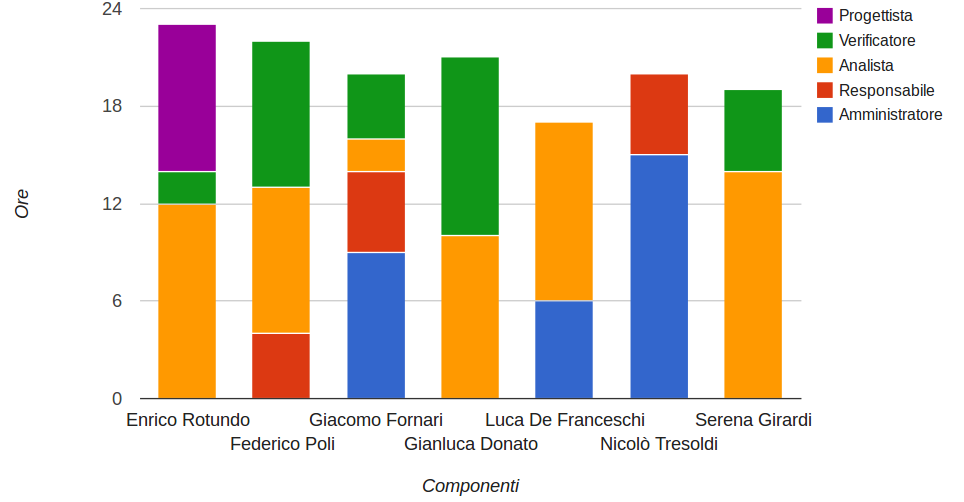
\includegraphics[scale=0.35]{4-1.png}
\caption{Ore per componente, fase di Analisi\label{fig:nome}}
\end{figure}

Si fa notare che le ore sopra indicate non sono incluse nelle 105 ore rappresentanti il tetto massimo di ore somministrabile da ciascun componente.

\subsection{Progettazione architetturale}

Nella fase di Progettazione architetturale ciascun componente dovrà rivestire i seguenti ruoli:

\begin{table}[H]
\centering
\begin{tabular}{lccccccccc}
\toprule 
    \textbf{Nome}  & \multicolumn{6}{c}{\textbf{Ore per ruolo}} & \textbf{Ore totali} \\
    & Amm. & Analista & Progettista & Prog. & Responsabile & Ver. \\
    \midrule
    Enrico Rotundo   	& 5 &  &	 15	& &   &	2 &	24 \\
    Federico Poli  		& 4	&  &	 15	& &   & 4 & 19 \\
    Giacomo Fornari		& 	&  &	 18	& &   &	12 & 30 \\
    Gianluca Donato 		& 	&  &	 25	& &   &	6 & 31 \\
    Luca De Franceschi 	& 	&  &	 18	& & 3 &	11 & 32 \\
    Nicolò Tresoldi 		& 	&  &	 21	& &   & 8 & 29 \\
   	Serena Girardi 		& 5	&  &	 21	& &   &	8 & 34 \\
    
    \bottomrule
\end{tabular}
\caption{Ore per componente, fase di Progettazione architetturale}
\end{table}
I valori in tabella sono riassunti nel seguente grafico: \\ \\ \\

\begin{figure}[H]
\centering
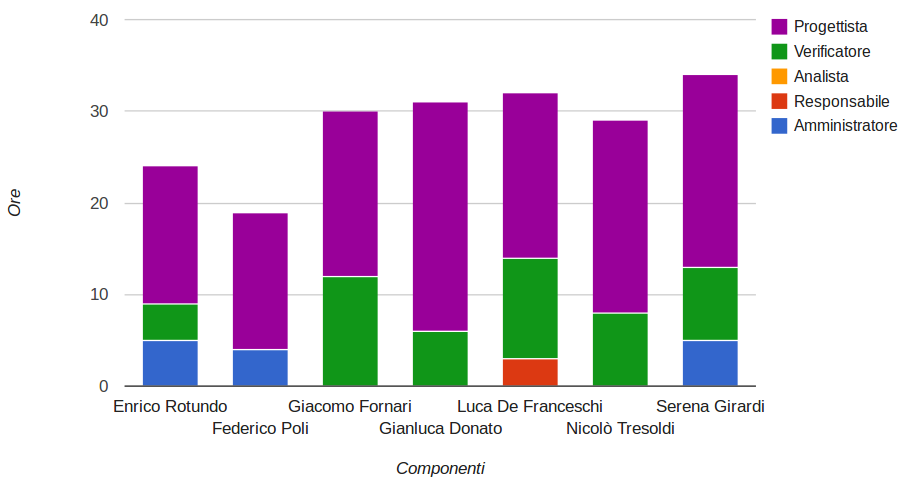
\includegraphics[scale=0.35]{4-2.png}
\caption{Ore per componente, fase di Progettazione architetturale\label{fig:nome}}
\end{figure}

\pagebreak
\subsection{Progettazione di dettaglio e codifica}

Nella fase di Progettazione di dettaglio e codifica ciascun componente dovrà rivestire i seguenti ruoli:

\begin{table}[H]
\centering
\begin{tabular}{lccccccccc}
\toprule 
    \textbf{Nome}  & \multicolumn{6}{c}{\textbf{Ore per ruolo}} & \textbf{Ore totali}\\
    & Amm. & Analista & Progettista
    & Prog. & Responsabile & Ver. \\
    \midrule
    Enrico Rotundo   	& 3 &  &	 10	& 35 & 6 & 10 &	64 \\
    Federico Poli  		& 7	&  &	 28	& 35 &   & 5  & 75 \\
    Giacomo Fornari		& 	&  &	 32	&    &   & 27 & 59 \\
    Gianluca Donato 		& 	&  &	 12	& 30 &   & 14 & 56 \\
    Luca De Franceschi 	& 16	&  &	 20	&    &   & 18 & 54 \\
    Nicolò Tresoldi 		& 	&  &	 12	& 30 &   & 19 & 61 \\
   	Serena Girardi 		& 	&  &	 12	& 30 & 4 & 17 & 63 \\
    
    \bottomrule
\end{tabular}
\caption{Ore per componente, fase di Progettazione di dettaglio e codifica}
\end{table}

I valori in tabella sono riassunti nel seguente grafico: \\ \\ \\

\begin{figure}[H]
\centering
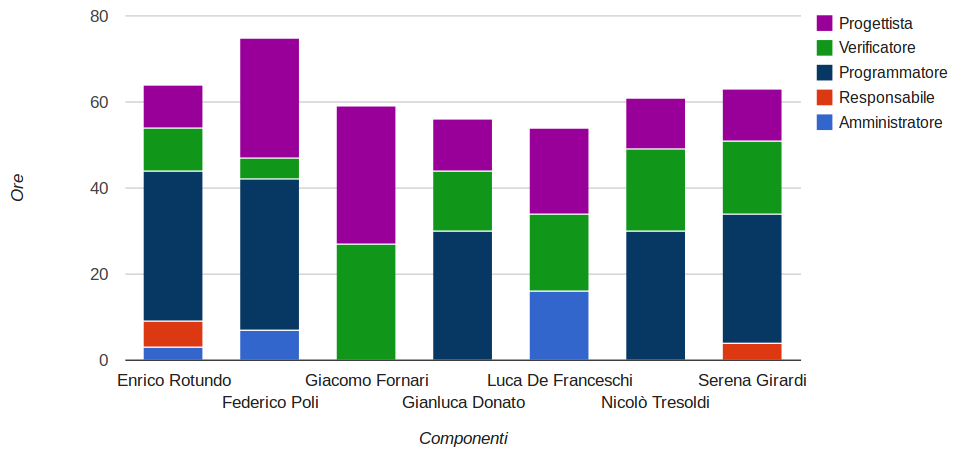
\includegraphics[scale=0.35]{4-3.png}
\caption{Ore per componente, fase di Progettazione di dettaglio e codifica \label{fig:nome}}
\end{figure}

\subsection{Validazione}

Nella fase di Validazione ciascun componente dovrà rivestire i seguenti ruoli:

\begin{table}[H]
\centering
\begin{tabular}{lccccccccc}
\toprule 
    \textbf{Nome}  & \multicolumn{6}{c}{\textbf{Ore per ruolo}} & \textbf{Ore totali}\\
    & Amm. & Analista & Progettista
    & Prog. & Responsabile & Ver. \\
    \midrule
    Enrico Rotundo   	&   &  &	 7	&   &   & 8 & 15 \\
    Federico Poli  		& 	&  &	 	&   &   & 8 & 8  \\
    Giacomo Fornari		& 	&  &	 	& 8 &   & 6 & 14 \\
    Gianluca Donato 		& 11	&  &	 	&   &   &   & 15 \\
    Luca De Franceschi 	& 	&  &	 5	& 8 &   & 5 & 18 \\
    Nicolò Tresoldi 		& 	&  &	 7	&   &   & 6 & 13 \\
    Serena Girardi 		& 	&  &	 	&   & 5 & 8 & 5  \\
    
    \bottomrule
\end{tabular}
\caption{Ore per componente, fase di Validazione}
\end{table}

I valori in tabella sono riassunti nel seguente grafico: \\ \\ \\

\begin{figure}[H]
\centering
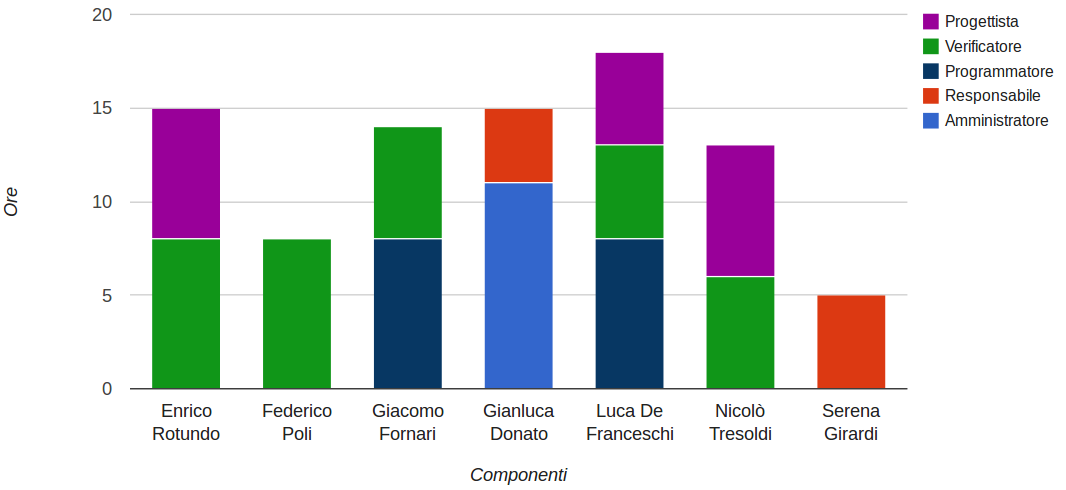
\includegraphics[scale=0.35]{4-4.png}
\caption{Ore per componente, fase di Validazione\label{fig:nome}}
\end{figure}

\subsection{Totale}

Il totale delle ore, comprensive delle ore di Analisi dei requisiti che saranno fornite da ciascun membro del gruppo nel corso dell'intero progetto sono le seguenti:

\begin{table}[H]
\centering
\begin{tabular}{lccccccccc}
\toprule 
    \textbf{Nome}  & \multicolumn{6}{c}{\textbf{Ore per ruolo}} & \textbf{Ore totali}\\
    & Amm. & Analista & Progettista
    & Prog. & Responsabile & Ver. \\
    \midrule
    Enrico Rotundo   	& 8 & 12& 41 & 35 & 6 & 24 & 126 \\
    Federico Poli  		& 11	& 9 & 43 & 35 & 4 & 22 & 124 \\
    Giacomo Fornari		& 9	& 2 & 50 & 8  & 5 & 49 & 123 \\
    Gianluca Donato 		& 11	& 10& 37 & 30 & 4 & 31 & 123 \\
    Luca De Franceschi 	& 22	& 11& 43 & 8  & 3 & 34 & 121 \\
    Nicolò Tresoldi 		& 15	&   & 40 & 30 & 5 & 33 & 123 \\
    Serena Girardi 		& 5	& 14& 33 & 30 & 9 & 30 & 121 \\
    
    \bottomrule
\end{tabular}
\caption{Ore per componente totali, inclusa fase di Analisi}
\end{table}

\begin{figure}[H]
\centering
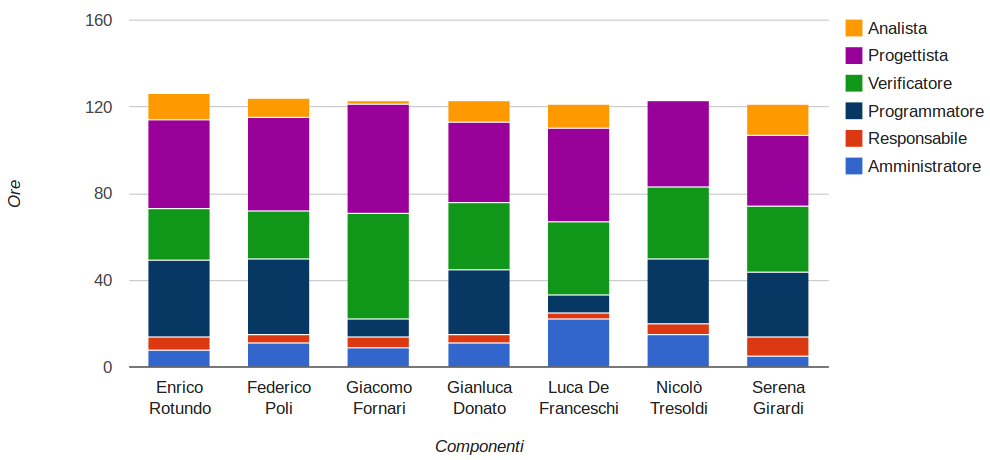
\includegraphics[scale=0.35]{4-5-1.png}
\caption{Ore per componente totali, inclusa fase di Analisi\label{fig:nome}}
\end{figure}

Nella seguente tabella sono invece riportate le ore fornite da ciascun componente, escluse quelle rientranti nella fase di Analisi dei requisiti. 
Le ore totali preventivabili devono essere comprese tra la soglia minima di 85 ore e quella massima di 105.

\begin{table}[H]
\centering
\begin{tabular}{lccccccccc}
\toprule 
    \textbf{Nome}  & \multicolumn{6}{c}{\textbf{Ore per ruolo}} & \textbf{Ore totali}\\
    & Amm. & Analista & Progettista
    & Prog. & Responsabile & Ver. \\
    \midrule
    Enrico Rotundo   	& 8 & & 32 & 35 & 6 & 22 & 103 \\
    Federico Poli  		& 11	& & 43 & 35 &   & 13 & 102 \\
    Giacomo Fornari		& 0	& & 50 & 8  &   & 45 & 103 \\
    Gianluca Donato 		& 11	& & 37 & 30 & 4 & 20 & 102 \\
    Luca De Franceschi 	& 16	& & 43 & 8  & 3 & 34 & 104 \\
    Nicolò Tresoldi 		& 0	& & 40 & 30 &   & 33 & 103 \\
    Serena Girardi 		& 5	& & 33 & 30 & 9 & 25 & 102 \\
    
    \bottomrule
\end{tabular}
\caption{Ore per componente totali, rendicontate}
\end{table}

\begin{figure}[H]
\centering
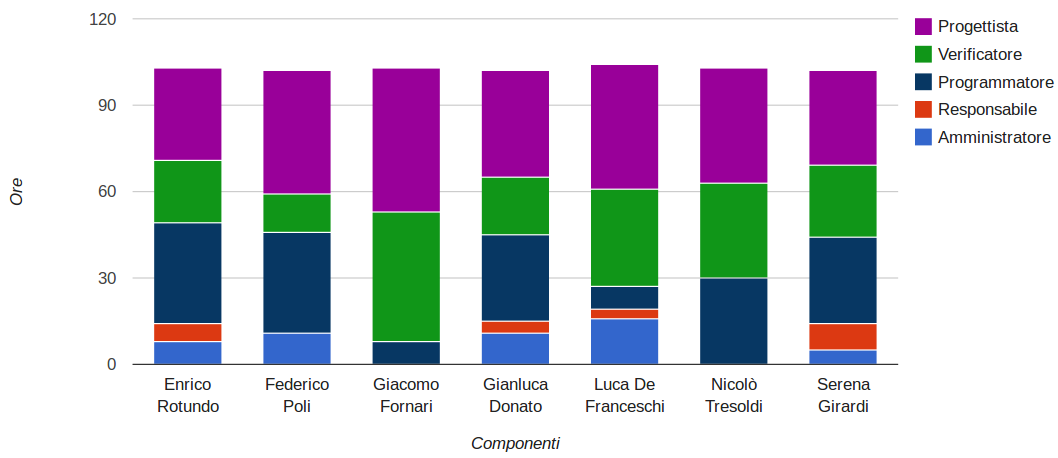
\includegraphics[scale=0.35]{4-5-2.png}
\caption{Ore per componente totali, rendicontate\label{fig:nome}}
\end{figure}